\chapter{Foundations and Related Work\label{cha:chapter2}}
This section formally discusses the state of the art machine learning techniques and strategies that have been used practically for chatbots.
\\~\\
In the current era, a lot of research is happening to make the chatbots to communicate like humans without being recognized as a machine. But in reality, a lot of development is still pending in this regard. Technological elevation using machine learning(ML) and artificial intelligence(AI) is helping this technology to get pushed forward through learning. At the same time, there are emerging challenges and problems hindering the pace of the progress. Many major companies are working to make an ideal agent but still are unable to produce one. 
% But with every new year it is getting more mature and the day is not so far when there will be a robot which can make humans wonder by communicating even better than the creators.
This chapter illustrates the initial purpose of introducing the chatbots and why there appeared a need for these agents? The basic and important chatbot classifications and techniques are introduced. In addition to that, the work and research accomplished so far under this area are featured. Let's start with a brief historical background about the chatbots. 
% chatbots definition and brief historical background.

\section{Chatbots History}
According to Shawar and Atwell (2007) initially, chatbots were introduced in the 1960s and the key idea behind it was to make the communication feel real like humans \cite{ChatbotsAreTheyReallyUseful}. In addition to it, as stated by Zadrozny et al. (2000) to make humans interact with the computers it can only be led by making humans "to express their interests, wishes, or queries directly and naturally by speaking, typing, and pointing" \cite{NaturLangDialPersInter}. For the accomplishment of such objectives, the chatbots were introduced \cite{ChatbotsAreTheyReallyUseful}. But now their applications are extended just like their scope. Mostly these artificial agents have covered the entertainment sector, information search, and assisting humans in the e-commerce and business sector. But when it comes to replicate human beings it is still one of the biggest challenges in the present. As an understanding of natural language, grabbing feelings, verbal structure, gestures, and body language just like living beings are the main hindrances for a machine to act like a human \cite{CreatingChatbotsToTalk}.    
\\~\\
Many companies claim for operating their chatbots and doing research on them. As mentioned on the website "botnerds.com"\cite{botnerds}, the stats for spring 2017 are as follows:
\begin{itemize}
\item Facebook alleges over 100,000 bots on Messenger.
\item Twitter claims approximately 48 million bot accounts.
\item Kik confesses 20,000 bots on its platform.
\item Wit.ai claims 21,500 workers for development.
\item Small amount of skype bots are also available.
\end{itemize}
The next section provides the technical knowledge of the dialogue systems. 

% Moreover, these bots can be classified according to their serving purpose.

% \subsection{Chatbots Classifications}
% The purpose of serving matters for chatbots to be judged as good or bad. 

% \subsubsection*{Good Chatbots}
% These chatbots lie under the category of agents used for informative purpose or social welfare. As follows \cite{botnerds}:
% \begin{itemize}
% \item Chat bots.
% \item Crawlers.
% \item Transactional bots.
% \item Informational bots.
% \item Entertainment bots: Art bots, Game bots.
% \end{itemize}

% \subsubsection*{Bad Chatbots}
% These are the bots having negative aspects and used for bogus purposes. Some are mentioned below\cite{botnerds}:
% \begin{itemize}
% \item Hackers.
% \item Spammers.
% \item Scrapers.
% \item Impersonators. 
% \end{itemize}
% Furthermore, if you dig deep into it you can figure out precisely the serving purpose of the bots which can be either political, representation i.e. me bots, searching, chatting, working e.g. slack bots used in many workplaces and voice communication. And some of the well known artificial agents like Alexa, Google Assistant, Siri, and Cortana are being used to serve these purposes for a long time \cite{listeningtobots}. Moreover, we can categorize the conversational bots based on functionalities that they are performing.

% \subsection{Chatbots Categories}
% It is not an easy task to categorize chatbots but according to the market and looking into the characteristics of the chatbots, they can be classified as mini bots also called "Specialist Bots" and complex bots having the ability to perform generally known as "Generalised Bots". \cite{botnerds}
% \\~\\
% In addition to that specialized bots are mainly the ones that are developed by a developer or small team of developers serving some specific domain. Whereas, generalized bots are those mainly produced by multinational firms and have the ability to perform in every aspect and somehow trying to mimic humans in communication.

% \begin{figure}[h]
%     \centering
%     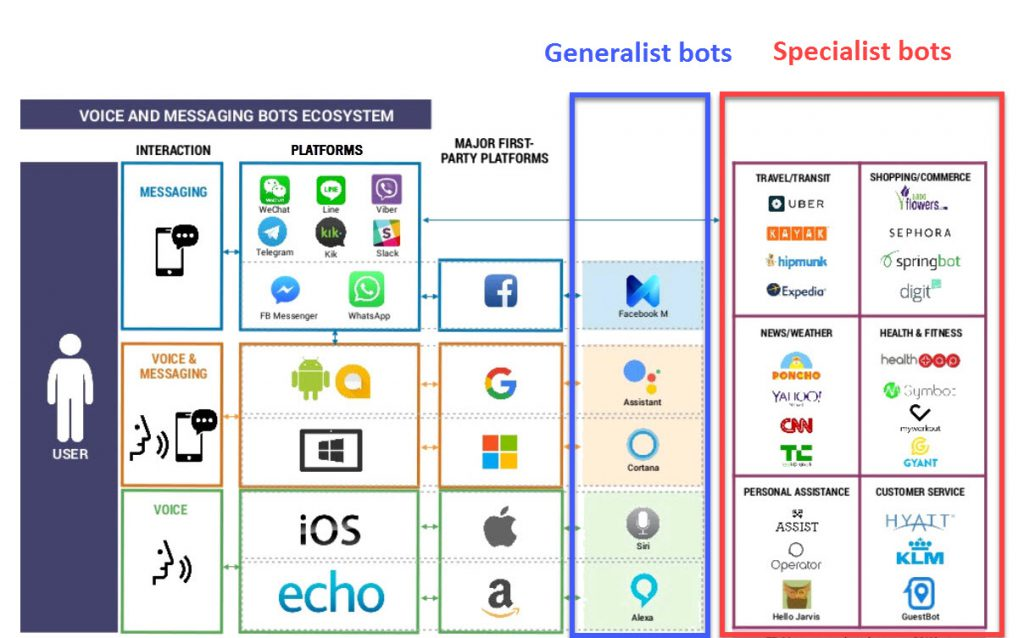
\includegraphics[width=0.9\textwidth]{img/generalist-vs-specialist.jpg}
%     \caption{Categorizing Generalized and Specialist Bots \cite{botnerds}}
%     \label{fig:ann}
% \end{figure}
% \\~\\
% Now digging into the generalized bots that how can they be built smart enough to deliver humanly. And then there comes a human characteristic which makes humans superior to other beings known as intelligence.

\section{Dialogue Systems}
The importance of human-computer interaction has raised drastically in the last few years. It is due to its rising potential towards solving daily life problems especially providing aid in commercial challenges. With the advancement of big data and machine learning, the self-functioning virtual assistant doesn't seem to be impossible. Jurafsky and Martin (2019) classified dialogue systems as (i) Systems designed to complete a task i.e. Task-oriented dialogue agents and (ii) Systems for extended unstructured conversation i.e. Chatbots \cite{dialogsysandchatbots}.
% So, based on the applications of conversation agents, the dialogue systems can be divided into two main categories i.e. Task-Oriented Systems and Non-Task Oriented Systems (chatbots).

\subsection{Task Oriented Agents}
These systems are designed to accomplish a task in some specific domain. The system interprets a message provided by the user, symbolizes it to the internal state, and processes it according to the state of the dialogue. Lastly, the final action is performed on it to produce a response \cite{surveyondialogsystems}. Common examples of such virtual agents are Apple's Siri, Google Home, and Amazon's Alexa.
\\~\\
Mainly natural language understanding is done using statistical models. On the other hand, some systems still use human-designed pre-defined rules for slot filling and detecting an intent \cite{surveyondialogsystems}. It not only results in more time consumption and makes deployment of such system costly, but also restricts the operational domain for the system. To overcome these challenges, deep learning played an important role.

% \subsubsection*{Pipeline Methods \label{sec:pipelineMethods}}
% As mentioned in \cite{surveyondialogsystems} Task-oriented systems consisting of pipeline methods inherit following four major components:
% \begin{itemize}
% \item Natural Language Understanding(NLU) to perceive the semantics of the user utterance.
% \item Dialogue state Tracker to supervise the dialogue history and return the recent dialogue state.
% \item Policy Learning to predict the upcoming action on the bases of the last dialogue state.
% \item Natural Language Generation(NLG) for transforming the respective action to the response represented as natural language.
% \end{itemize}
% Graphical representation of pipeline methods has shown below in Figure \ref{fig:to}. 
% \begin{figure}[h]
%     \centering
%     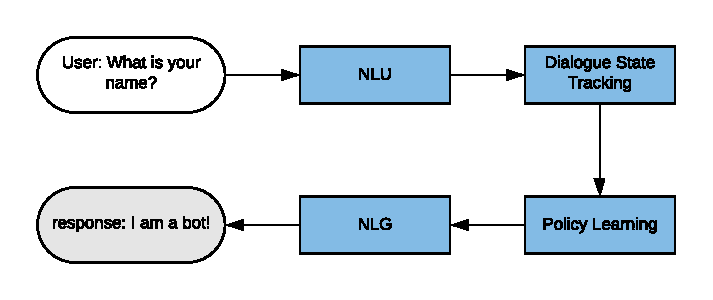
\includegraphics[width=0.9\textwidth]{img/Task_oriented.pdf}
%     \caption{Process for Task Oriented Dialog Systems \cite{surveyondialogsystems}}
%     \label{fig:to}
% \end{figure}
% \\~\\
% Pipeline based task-oriented systems need a lot of spoon-feeding in a particular domain, making them hard to adjust with new domains \cite{surveyondialogsystems}. In addition to that, the inter-dependency of the components also refrains the system to adapt to the new environment. To neglect these challenges end-to-end based task-oriented systems have been proposed \cite{surveyondialogsystems}. 
% \\~\\
% % \subsubsection*{End-to-End Methods}
% Unlike the pipeline system, the end-to-end system consists of a single module and collaborates with large structured databases \cite{surveyondialogsystems}. These methods lie under the domain of neural generative models which are discussed below in the section of non-task oriented systems(chatbots). Many practices have already been made to design a framework for task-oriented dialog systems having end-to-end specifications using end-to-end neural generative methodologies \cite{surveyondialogsystems}. 
\\~\\
Modern task-oriented dialogue systems are based upon the following architectures:
\subsubsection*{Frame-based Architecture}
Jurafsky and Martin (2019) narrates that state-of-the-art task-oriented dialogue systems are composed of frames. The information extracted from the user utterances by the system to identify the intentions of the user is stored in the form of a knowledge structure which is known as a frame. The slot could be a key-value pair of some specific type and a frame is composed of a group of such slots. These slots indicate what information is required by the system. Once these slots get filled then the system can perform some action accordingly \cite{dialogsysandchatbots}. Example of a frame along with the slots and their types and question to fill each slot has been shown in Figure \ref{fig:frame}.

\begin{figure}[h]
    \centering
    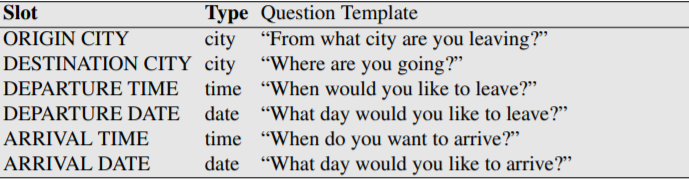
\includegraphics[width=0.9\textwidth]{img/frame.PNG}
    \caption{A frame showing each slot along with its type and related question. \cite{dialogsysandchatbots}}
    \label{fig:frame}
\end{figure}

\subsubsection*{Dialogue-state Architecture}
It is the most refined form of frame-based architecture. It is also named as belief-state architecture \cite{dialogsysandchatbots}. Whenever there comes a new user utterance, the NLU component extracts the required knowledge to fill the related slots. Secondly, the dialogue manager includes dialogue state tracker which is responsible for tracking and handling the entire dialogue information and values for each slot of a frame. Whereas, the policy learning component is responsible for deciding on the further action that the system should perform or convey. Once the dialogue policy confirms that what action should be taken by the system according to the updated dialogue state. Afterward, Natural Language Generation(NLG) component takes an action to produce the textual response for the users \cite{surveyondialogsystems}. Graphical representation of such architecture is shown in Figure \ref{fig:dms}.    

% The components for the conventional dialogue-state systems have been shown in Figure \ref{fig:to}.
% \begin{figure}[h]
%     \centering
%     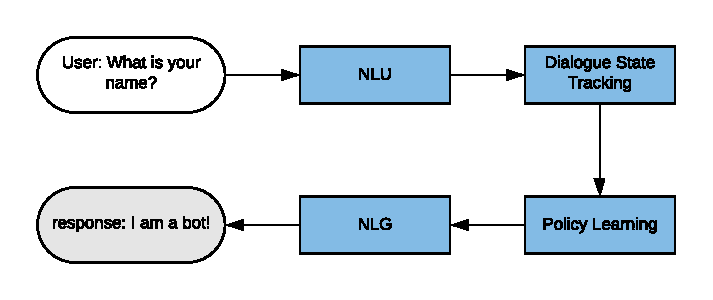
\includegraphics[width=0.9\textwidth]{img/Task_oriented.pdf}
%     \caption{Dialogue-state architecture for task-oriented system \cite{surveyondialogsystems}.}
%     \label{fig:to}
% \end{figure}

\subsection{Chatbots}
Chatbots are considered to be the simplest form of the dialogue systems \cite{dialogsysandchatbots}. The main goal of such systems is to communicate with humans on any topic without restricting it to some specific domain, making them more independent and self-sustainable. Applications of such a system are entertainment or general conversation with meaningful responses \cite{surveyondialogsystems}.
\\~\\
Furthermore, chatbots can also be categorized based on their composition design and methodology used for language processing. Jurafsky and Martin (2019) classified the chatbots into two divisions: (i) Rule-based chatbots and (ii) Corpus-based chatbots \cite{dialogsysandchatbots}.

\subsubsection*{Rule-based Chatbots}
Such conversational agents are trained on simple rules to communicate. There are pre-defined actions for which the user is provided with a choice of selection. These conversational agents mainly include questions to which the user can agree or disagree. Other than that they are also capable of detecting a keyword or a group of terms to proceed further and generate a proper response for the user utterance. ELIZA and PARRY are the most common examples of the chatbots that followed the rule-based approach \cite{dialogsysandchatbots}.  

\subsubsection*{Corpus-based Chatbots}
Unlike rule-based agents, these are capable of learning and getting trained for general dialogue. For this reason, they need a humongous data source for getting trained enough to perform general conversation like humans. As stated by Serban et al. (2018) that a chatbot could need hundreds of millions or billions of words for sufficient training \cite{surveyofavailablecorpora}. Once they are operational, these agents are also capable of self-learning, and user responses and utterances can also be used as additional data for training purposes \cite{dialogsysandchatbots}. The dialogue framework implemented under the scope of this master's thesis is capable of getting trained for the provided training corpus but the ability to use users' utterances as training data could be added in the future.
\\~\\
The next section explains the means that could be adapted by the users to interact with the dialogue systems.

\section{Communication Channels}
There are two types of communication channels that almost all the chatbots are using for communication i.e. messaging platforms for text messages like Slack and speech communication platforms like Alexa \cite{frameworkforunderstandingchatbots}. 

\subsubsection*{Text}
These chatbots use text messages for communication. They have an extra advantage as the input and output are in the textual form which is easier to understand, store, and adapt.

\subsubsection*{Speech}
Chatbots with voice or speech feature support is more user convenient and provide a more realistic and natural mean of communication as they take input using vocals and produce spoken output. 

\subsubsection*{Text and Speech}
There also exist such chatbots that have the conversational support using both voice and text channels. They provide the user with an option to configure the way of taking input and expressing the output \cite{frameworkforunderstandingchatbots}.
\\~\\
The dialogue framework developed in this master's thesis only supports textual input for now. Support for interaction via both manners (text and speech) could be integrated into the next version of the system.
% Moreover, the corpus-based systems are mainly designed by utilizing the following methodologies: (i) Retrieval-based methods, (ii) Generative methods, and (iii) Hybrid methods. These methods have been discussed ahead in the section 

 
% According to Peters (2018) multiple components combine to build a chatbot. Whenever there comes any message from the user, it directly passes to the language identification module. It varies from simple tag retrieval to more elaborate statistical methods like n-gram models \footnote{\url{https://en.wikipedia.org/wiki/N-gram}}. The new message along with the language and potential previous conversation messages retrieved from the database are then pushed to the intent classifier module which identifies the user's conveyed intent. Eventually, a fitting action or a series of actions is produced using the message’s metadata, identified intent, and other related information from the database. Lastly, the action or a sequence is passed to the action handler module as input and after its execution, it generates an appropriate response \cite{designandimplementation}.  Diagrammatic overview for rule-based chatbots has been displayed in Figure \ref{fig:chatbotDiagOverv}.
% \begin{figure}[h]
%     \centering
%     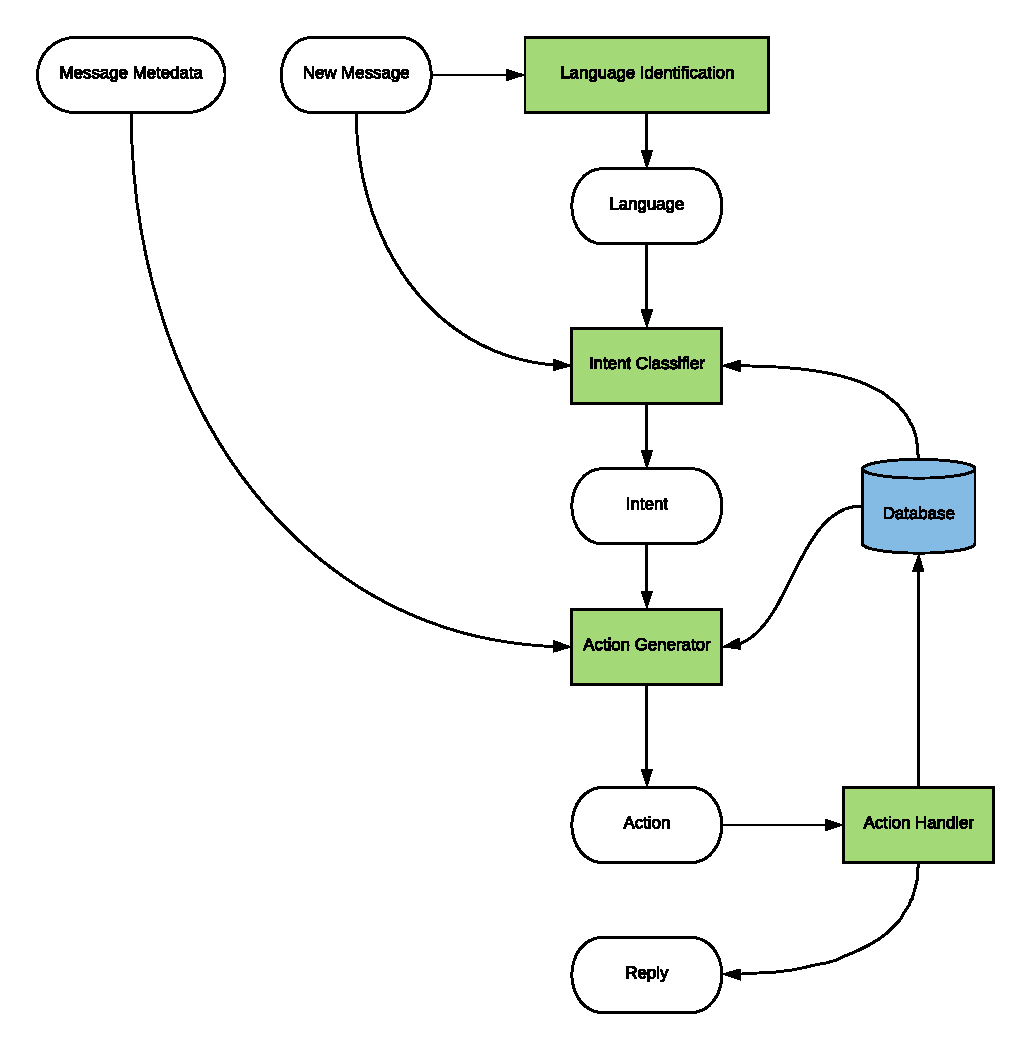
\includegraphics[width=0.9\textwidth]{img/overview.pdf}
%     \caption{diagrammatic overview \cite{designandimplementation}}
%     \label{fig:chatbotDiagOverv}
% \end{figure}


% Next section explains the high-level representation of the chatbots. 

% \subsection{Chatbots}
% Chatbots are the basic dialogue systems that are designed to carry out the conversation. 
% \\~\\
% According to Jurafsky and Martin (2019) chatbots can be classified 

% \subsection{Chatbots Overview}
% % \section{Dialogue Systems}
% Concertedly, multiple components combine to build a chatbot. Whenever there comes any message from the user, it directly passes to the language identification module. The new message along with the language and potential previous conversation messages retrieved from the database are then pushed to the intent classifier module which identifies the user's conveyed intent. Eventually, a fitting action or a series of actions is produced using the message’s metadata, identified intent, and other relevant information from the database. Lastly, the action or a sequence is passed to the action handler module as input and after its execution, it generates an appropriate response. \cite{designandimplementation} 
% \\~\\
% Its diagrammatic overview has been displayed in Figure \ref{fig:chatbotDiagOverv} below.
% \begin{figure}[h]
%     \centering
%     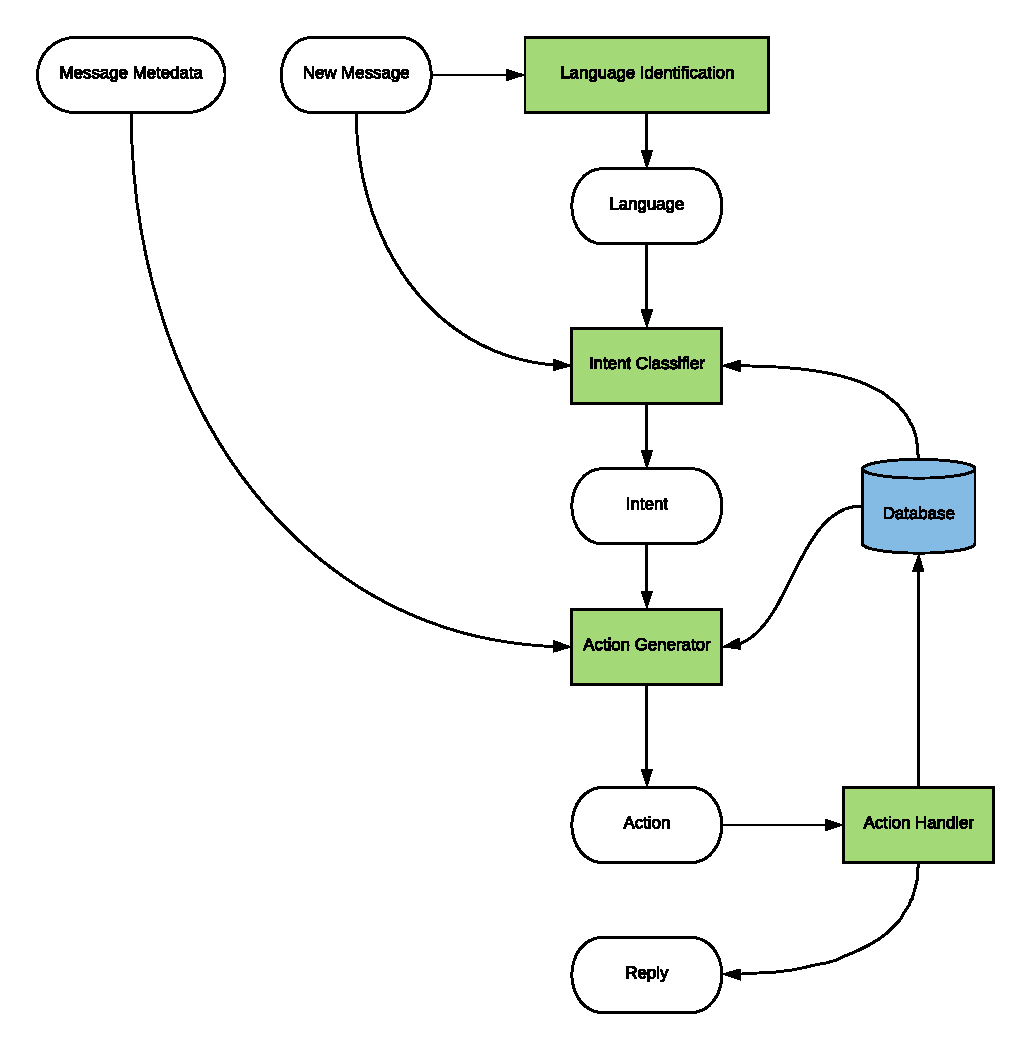
\includegraphics[width=0.9\textwidth]{img/overview.pdf}
%     \caption{Chatbots diagrammatic overview \cite{designandimplementation}}
%     \label{fig:chatbotDiagOverv}
% \end{figure}


% \subsection{Technical Background}
% This section explains the technical knowledge about chatbots.
% \\~\\
% According to Peters(2018) multiple components combine to build a chatbot. Whenever there comes any message from the user, it directly passes to the language identification module. It varies from simple tag retrieval to more elaborate statistical methods like n-gram models \footnote{\url{https://en.wikipedia.org/wiki/N-gram}}. The new message along with the language and potential previous conversation messages retrieved from the database are then pushed to the intent classifier module which identifies the user's conveyed intent. Eventually, a fitting action or a series of actions is produced using the message’s metadata, identified intent, and other related information from the database. Lastly, the action or a sequence is passed to the action handler module as input and after its execution, it generates an appropriate response \cite{designandimplementation}.

% Its diagrammatic overview has been displayed in Figure \ref{fig:chatbotDiagOverv} below.
% \begin{figure}[h]
%     \centering
%     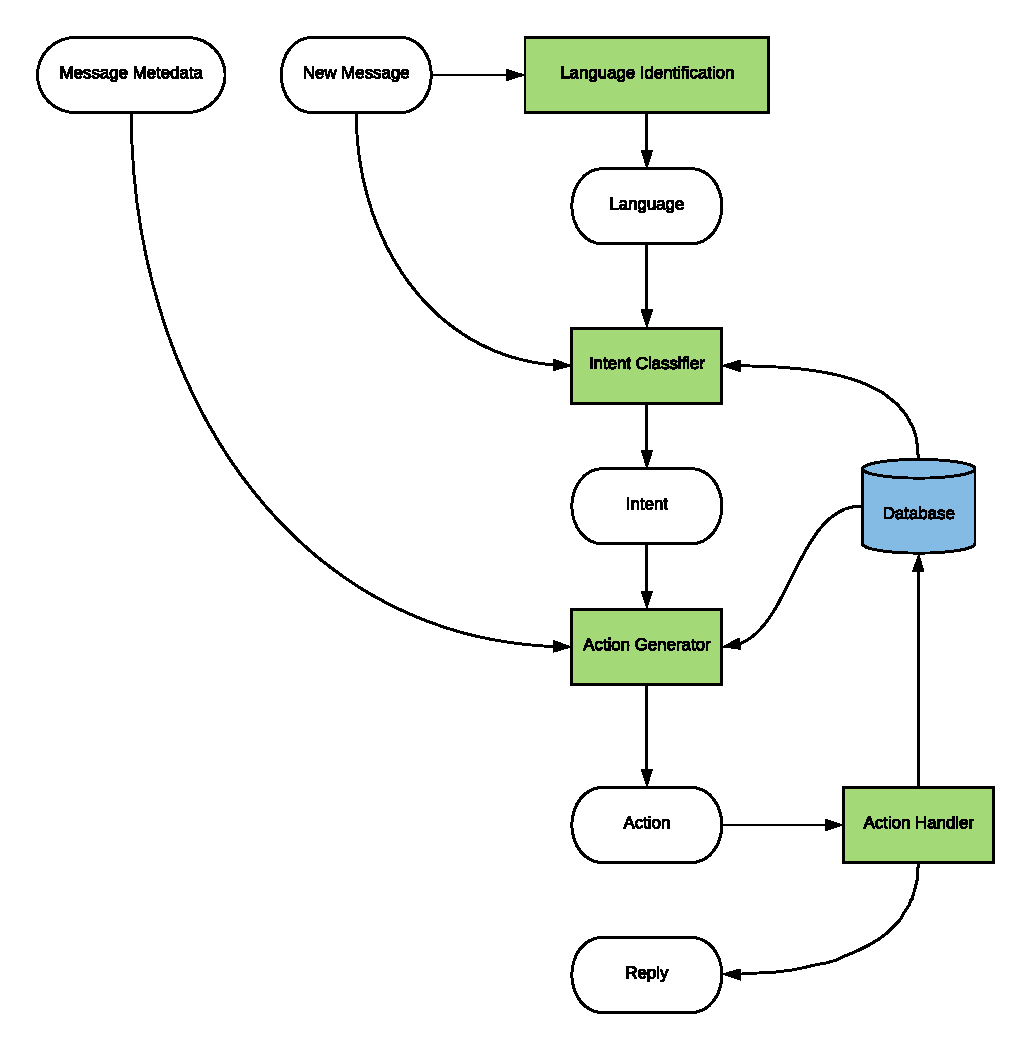
\includegraphics[width=0.9\textwidth]{img/overview.pdf}
%     \caption{Chatbots diagrammatic overview \cite{designandimplementation}}
%     \label{fig:chatbotDiagOverv}
% \end{figure}
% \\~\\
% When it comes to Natural Language Processing, Word Embedding and Recurrent Neural Networks are commonly used techniques for deep learning. Furthermore, Intent classification can be done using a variety of techniques that vary from Simple Keyword Extraction to Bayesian Inference. Afterward, the response can be generated using retrieval-based and generative-based methods \cite{designandimplementation}.  
% \\~\\
% One of the most important components for a chatbot is dialogue management. Initial technical approaches for a dialogue manager had been characterized as a dialogue grammar, a plan-based approach, or a collaborative approach \cite{dialoguemanagementsystems}\cite{spokenDialogueTechnology}. Currently, advanced approaches known as statistical methods are helpful for the enhancement of strategies for dialogue management \cite{statisDialManag}. These models can get trained using substantial dialogues providing robustness to the system \cite{statisDialManag}. The type and amount of knowledge implemented in the manager, the distribution of tasks between the system and the user, and the system's meta-communication (confirmation, clarification, repair, and recovery) strategies are the most essential attributes of the dialogue manager \cite{subjectiveQualityEvaluation}.
% ________________________
% \section{Bots Intelligence}
% To inject intelligence into the bots firstly, one should know what is it. So for this reason, a man generated some mathematical models resembling human brain architecture and tried to train them and made those models learn by providing some sample information or data. For making the bots intelligent one has to use these models. All existing smart bots use machine learning(ML) and artificial intelligence(AI) techniques to comprehend the language, complex task processing and to figure out the best response. \cite{botnerds}
% \\~\\
% based on the intelligence, bots can be segregated. Some bots use and are dependent on ML and AI is known as "Smart Bots". Those without any AI can be put under the category of "Script Bots" as the just use a script and are dumb without it. \cite{botnerds}
% \\~\\
% Furthermore, AI can also be divided as weak or strong. Weak AI includes pre-defined rules and scopes to make the chatbots work in the right direction. Whereas, the strong one is free from such pre-declared rules and can learn different behaviors on its own. \cite{CreatingChatbotsToTalk}



\section{Chatbots Components and Tasks}
Chatbots consist of various components and each component is responsible for performing a specific task. Usually, a chatbot is composed of the following components:
\begin{itemize}
    \item Speech to Text Converter.
    \item Natural Language Processor.
    \item Response Generator.
    \item Knowledge Base.
    \item Dialogue Manager.
    \item Text to Speech Synthesizer.
\end{itemize}
As already mentioned in the previous section that the conversational agent developed in this master's thesis is only capable of taking input in textual form. The very first component i.e. speech to text and the last one i.e. text to speech are only applicable if there is an involvement of speech. So these two elements are overlooked in this research. Other than that rest of the components are discussed below. 
\\~\\
Starting with natural language processing(NLP), it plays an important role in dialogue systems to understand the semantics of the inputted text and is also responsible for detecting the intents and entities. Moreover, intent and entity classification could be done using a variety of techniques that vary from Simple Keyword Extraction to Bayesian Inference. Afterward, the response could be generated using retrieval-based and generative-based methods \cite{designandimplementation}.  
\\~\\
Once the response has been generated, it is passed to the dialogue manager which is responsible to manage the dialogue as a whole. It decides how and what to respond to the user. Initial technical approaches used for dialogue management had been characterized as a dialogue grammar, a plan-based approach, or a collaborative approach \cite{dialoguemanagementsystems}\cite{spokenDialogueTechnology}. Currently, advanced approaches known as statistical methods are helpful for the enhancement of strategies for dialogue management \cite{statisDialManag}. These models can get trained using substantial dialogues providing robustness to the system \cite{statisDialManag}. Knowledge management, dialogue state, and response handling are the fundamental tasks for a chatbot. The system's meta-communication (confirmation, clarification, repair, and recovery) strategies are also the major attributes of the dialogue manager \cite{subjectiveQualityEvaluation}.

% \subsection{Language Identification}
% When it comes to a larger scale and diverse natural language processing then recognizing the language of a text is a necessary initial step. Some languages contain homographs i.e. Same words with different meanings. It is a challenging task for an algorithm to understand and grab the correct semantics if a language is not known beforehand. \cite{designandimplementation}
% \\~\\
% It is assumed for this master's thesis that messages will be provided using one language only. Despite it, there exist methods for inferring different languages in a single document or piece of text and can be found in the document \cite{multilanguagedetection}.
\subsection{Natural Language Processing(NLP)}
It is an essential chatbot element. NLP is a technical process for a better understanding of a user's utterance. It makes the chatbots to comprehend the semantics and the user intention behind the conversation. It is used to add more humanly characteristics to a chatbot and to make the dialogue feel more realistic. By adding NLP to a chatting agent, it becomes capable of learning and getting trained for any type of query or command provided by the user. Some methods for mastering the semantics of the text and for deep learning are discussed underneath. 
% Word Embedding and Recurrent Neural Networks are commonly used techniques for deep learning in this regard \cite{deepLearnBasedNLP}. 

% \subsubsection*{Deep Learning Techniques}
% In this section some commonly used deep learning will be explained that are used for Natural Language Processing(NLP). Word Embedding and Recurrent Neural Networks are frequently used techniques for deep learning \cite{deepLearnBasedNLP}. Furthermore, Intent classification can be done using a variety of techniques that vary from Simple Keyword Extraction to Bayesian Inference. Afterward, the response can be generated using previously discussed retrieval-based and generative-based methods.
\subsubsection*{Dialogue Act Detection}
Determining the function of the text whether it is a question, command, suggestion or an offer is known as dialogue act detection. It is one way of deriving semantics from natural language \cite{ciTalktosmartdev}\cite{archDesDev}. For a better understanding of it, an example has been shown in Figure \ref{fig:dade}.

\begin{figure}[h]
    \centering
    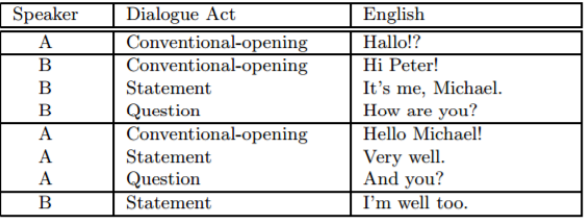
\includegraphics[width=0.9\textwidth]{img/Dialogue_Act.PNG}
    \caption{Dialogue act detection example \cite{archDesDev}.}
    \label{fig:dade}
\end{figure}

\subsubsection*{Intent and Entity Classification}
It is another way of understanding the meaning of the text represented in the form of natural language. Domain-specific dialogue acts are known as intents. An intent represents the user's real intention and goal of what he/she is trying to convey. Whereas, entities are modifiers for an intent. Entities could also be referred to as slots. Based on the detected intent the user can be directed further to available dialogue options \cite{sluSys}. 
\\~\\
Using NLP, a conversational agent can classify an intent and entity(s) in a user utterance. The main idea behind it for a chatbot is to detect the purpose of a talk that the user is trying to convey. For identification, the multi-classification problem is usually solved by labeling the utterances according to the possible user intentions and providing some relative names to them. Furthermore, there exist some techniques to complete this task varying from simple keyword extraction to Bayesian inference. These methods are meant to identify the user's request with the help of various messages. Well known LSTM\cite{lstm} networks are used to perform this task due to their high performing and delivering capacity \cite{intentclassificationusinglstm}.

\subsubsection*{Information Extraction}
Using this method for grasping the semantics, the unstructured text is transformed into structured grammar and passed to dialogue manager for further processing \cite{archDesDev}. 
\\~\\
As stated by McTear et al. (2016) that the initial step for information extraction is to break down the sentence or utterance into tokens. This process is named as tokenization. It is not an easy task to perform due to several challenges:
\begin{itemize}
    \item Phrases consisted of multiple terms e.g. the United States.
    \item Abbreviations e.g. U.S.A
    \item Contractions e.g. I'm
\end{itemize}
There are several techniques available to perform tokenization as mentioned in \cite{archDesDev}: (i) Bag of words, (ii) Latent Semantic Analysis, (iii) Regular Expressions, (iv) Part of Speech Tagging, (v) Named/Relation Entity Recognition, (vi) Semantic Role Labeling and (vii) Creation of Grammatical Data Structures. There also exist some statistical methods to extract the semantical information for the text as stated below:
\begin{itemize}
    \item Hidden Vector State Model \cite{semProhvsm}.
    \item Support Vector Machine Model \cite{svmModel}.
    \item Conditional Random Field Models \cite{crf}.
\end{itemize}

\subsubsection*{Deep Learning Techniques}
In this section, some commonly used deep learning will be explained that are used for Natural Language Processing(NLP). Word Embedding and Recurrent Neural Networks are frequently used techniques for deep learning \cite{deepLearnBasedNLP}.

\paragraph*{Word Embedding}
Word embedding technique is used for transforming words in the form of vectors \cite{designandimplementation}. These mapped vectors can be directly featured in machine learning algorithms. Different methods have already been introduced to exercise this operation. These approaches varies from simple vector count to statistical methods such as Word2Vec \cite{word2vec}, GloVe \cite{glove} and Skip-gram Model \cite{skipgram}. 

\paragraph*{Recurrent Neural Networks}
Recurrent Neural Networks(RNNs) are the neural networks specifically designed for sequenced data. More precisely, such networks work recursively having an internal state denoted as \texorpdfstring{C\textsubscript{t}}{C t} at a specific time t. Which is passed as an input to the neuron as upcoming time-step and it outputs a value \texorpdfstring{h\textsubscript{t}}{h t} based on \texorpdfstring{C\textsubscript{t}}{C t} at that time-step. But while implementing a simple RNN there comes gradient problems already proven by Mikolov et al. (2012) in “Understanding the exploding gradient problem” \cite{gradientproblem}. So to overcome this problem various revised methods have been introduced. According to \cite{designandimplementation} most commonly used ones are mentioned below: 
\begin{itemize}
\item Long Short Term Memory Units \cite{lstm}.
\item Gated Recurrent Units \cite{gru}.
\end{itemize}

\subsection{Response Generation \label{sec:respgen}}
Once the NLP component is done with its part then the gathered information is passed to the response generator. It is responsible to generate some meaningful responses to make the communication effective. So, for this purpose, a bot must reply coherently according to the context of the conversation. This challenging task is executed using the following pair of modules \cite{designandimplementation}:
\begin{itemize}
\item Module to provoke a list of competitive responses.
\item Module to select the most relevant reply based on some weighted value or specific metrics.
\end{itemize}
Moreover, there exist the following methods that are used practically to generate a response.
% to pass it to dialogue manager to take the end decision  
\subsubsection*{Retrieval-based Methods}
These methods consist of a humongous database containing successive responses. Chatbots developed employing such techniques contain the data structures like directed graphs and trees. The bot is competent enough to fetch the best response out of the numerous collection of responses. It is done by fetching the responses for the identified intents and entities related to the information provided in the form of a message. The information provided can usually be a regular expression searching for a specific structure of sentences or any output from the machine learning algorithm \cite{designandimplementation}. Whereas, such methods cannot self generate a natural language response like humans. Responses are either fed manually or via an already available knowledge base.

\begin{figure}[h]
    \centering
    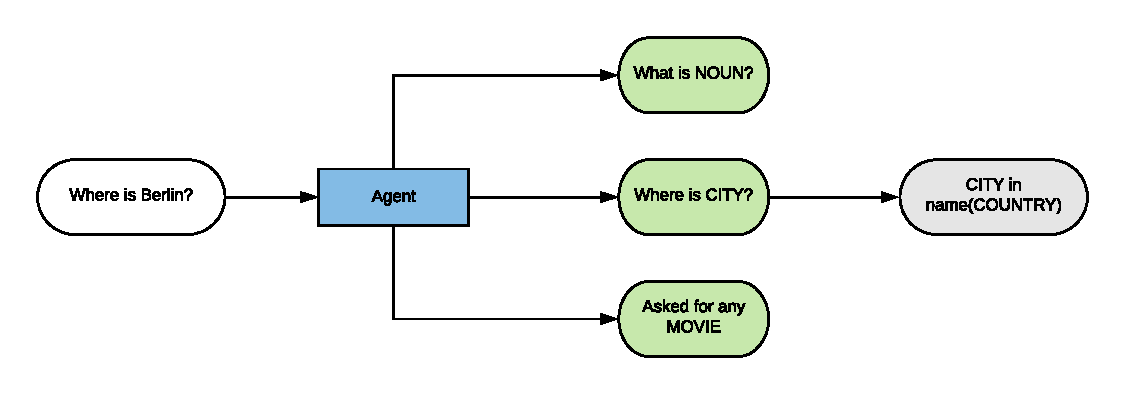
\includegraphics[width=0.9\textwidth]{img/Retrieval_based.pdf}
    \caption{Retrieval-based Methods Example \cite{designandimplementation}}
    \label{fig:rbm}
\end{figure}
\\~\\
The primary and fundamental step to achieve the retrieval-based method is message and response matching \cite{surveyondialogsystems}. The basic purpose of matching algorithms is to minimize the semantics difference between the responses and the messages \cite{surveyondialogsystems}. Two such techniques are mentioned below:
% \subparagraph*{Single Turn Response Matching}
\paragraph*{Single Turn Response Matching}
In this type of matching the only responsible factor for response generation is the message itself. Message context and successive answers are represented as a vector \cite{surveyondialogsystems}. 
% \subparagraph*{Multi Turn Response Matching}
\paragraph*{Multi Turn Response Matching}
Unlike single turn matching, current utterance along with all past messages are responsible for producing the most suitable response that best matches the overall context of the conversation \cite{surveyondialogsystems}.

\subsubsection*{Generative Methods}
Unlike retrieval-based methods, agents composed of generative models don't need pre-generated responses. They are capable of producing a new response based on the user's utterance using generative models. For generating a suitable response the model must be trained enough. Unfortunately, the performance of these models is still not sufficient enough to attract the companies due to various restrictions forced by the corporate \cite{designandimplementation}. The basic method for neural generative models has been briefly discussed below:

\begin{figure}[h]
    \centering
    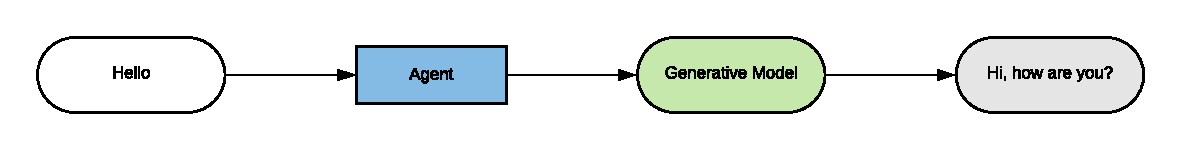
\includegraphics[width=0.9\textwidth]{img/Generative_based.pdf}
    \caption{Generative-based Methods Example \cite{designandimplementation}}
    \label{fig:gbm}
\end{figure}

\paragraph*{Sequence-to-Sequence Models}
Neural networks are being used by these models to symbolize dialog history and to produce useful responses \cite{surveyondialogsystems}. The systems based on these models don't need much knowledge base and pre-defined rules to generate natural language responses.
\\~\\
% Next section will cover the basis of neural generative models i.e. sequence-to-sequence models. After that, there will be explained some research topics underlying these models. 
% \cite{surveyondialogsystems}
Furthermore, Jiliang et al. (2017) mentioned some challenges that need to be discussed for generative-based methods:
\\~\\
% \paragraph*{Dialogue Context}
\textit{Dialogue Context}; To keep track of the current state of chatbot and recent conversation, it is compulsory to take care of the dialogue history and recent user utterances. It helps in understanding the context of dialogues to generate an appropriate response. Recurrent Neural Networks(RNN) are mainly used for this purpose.
% \cite{surveyondialogsystems}
\\~\\
% \paragraph*{Response Diversity}
\textit{Response Diversity}; To handle response diversity is a challenging task in the systems based on sequence-to-sequence models. As they can provide irrelevant, balanced, or completely related answers having some meaning. Inverse Document Frequency(IDF) is mainly used for this purpose.
\\~\\
% \paragraph*{Topic and Personality}
\textit{Topic and Personality}; The topic and personality of the dialogues is another factor to enhance their diversity. By acquiring the fundamental characteristics of dialogues, diversity can be increased and also it leads to gain consistency.  
\\~\\
% \paragraph*{Knowledge Base}
\textit{Knowledge Base}; For making the virtual assistant perform as humans do there is an essential need of a knowledge base. Not only using outside knowledge base we can cut the informational difference between machines and humans, but can also plant sensibility to artificial conversational agents.  
\\~\\
% \paragraph*{Interactive Learning}
\textit{Interactive Learning}; Eventually the main objective of a dialog system is to be smart enough to do self-learning during an interaction with a user.
\\~\\
% \paragraph*{Evaluation}
\textit{Evaluation}; In the end, the final step is to assess the provoked response quality generated using response generators. Task-oriented dialogue systems can be graded using handcrafted methods like ratings from the user. Whereas, for non-task oriented dialogue systems it is a bit challenging task to evaluate them. METEOR, BLEU, and ROGUE are some word overlap metrics to weigh the produced response quality \cite{surveyondialogsystems}.     

\subsubsection*{Hybrid Methods}
Hybrid approaches by combining both the above-mentioned methodologies have recently been introduced. If response generation fails using retrieval-based methods then it should be produced using generative-based methods. Retrieval based systems give more accurate results but that could be slow and vague \cite{surveyondialogsystems}. Whereas, neural generative systems can respond rapidly with the chance of giving useless results \cite{surveyondialogsystems}. So by unifying both of these methods, the performance can be enhanced significantly. More studies about these methods can be found in \cite{generateifnotretrieve}.

\subsection{Knowledge Base Designing and Management}
The intelligence of a chatbot is directly proportional to the knowledge available for its training and related processing \cite{archDesDev}. The knowledge base includes the bulk of training data for training of generative-based systems and the cluster of responses for retrieval-based conversational agents. Knowledgebase designing and management means how mature is the data gathered for training and managed to construct a corpus for the statistical dialogue systems. Making a chatting agent interact like humans also depends upon how well the corpus is designed and managed.
\\~\\
Cahn (2017) illustrates that at the beginning of this century humanly designed data corpuses served the purpose on a large scale. But over time, more advanced techniques have been introduced for collecting the data to design a knowledge base for chatbots. Currently, data scraping technique\footnote{\url{https://www.targetinternet.com/what-is-data-scraping-and-how-can-you-use-it/}} has provided ease by enabling data auto-collection over a large number of dialogues available on the web. By auto importing such a large amount of information, the knowledge corpora for the chatbots could also be auto-generated \cite{archDesDev}.
\\~\\
In present, Web API calls and optimized requests to the databases are extensively used to perform knowledge management \cite{designandimplementation}. Whereas, knowledge bases could also be represented as impressive graph-structured ontologies \cite{knowledgebase}.
\\~\\
There could be many data sources available for collecting data to manufacture knowledge base for chatbots. Some of them discussed in \cite{archDesDev} are:

\subsubsection*{Human-Annotated Collections}
Human-annotated dialogues could be modified to Artificial Intelligence Markup Language(AIML)\footnote{\url{https://en.wikipedia.org/wiki/AIML}} and other formations suitable for chatbots.

\subsubsection*{Discussion Forums}
Scraping online discussion forums can be helpful to serve the required purpose.

\subsubsection*{Email Messages}
Gathering data using email conversations could also result in the designing of a knowledge base.

\subsection{Dialogue Management}
Once the response generator component is done with its part then it passes the response to dialogue manager. It is responsible to manage the whole dialogue and checks according to the current state of dialogue whether to respond or not and what to respond to the user. Detailed architecture for a dialogue management system and data stream has been displayed in Figure \ref{fig:dms}. Components involved in dialogue management have been already explained before in the section "Dialogue-state Architecture". In addition to that, a dialogue manager is also liable for applying communication strategies along with the shaping of generated response to grant it real human-like sensation \cite{archDesDev}.

\begin{figure}[h]
    \centering
    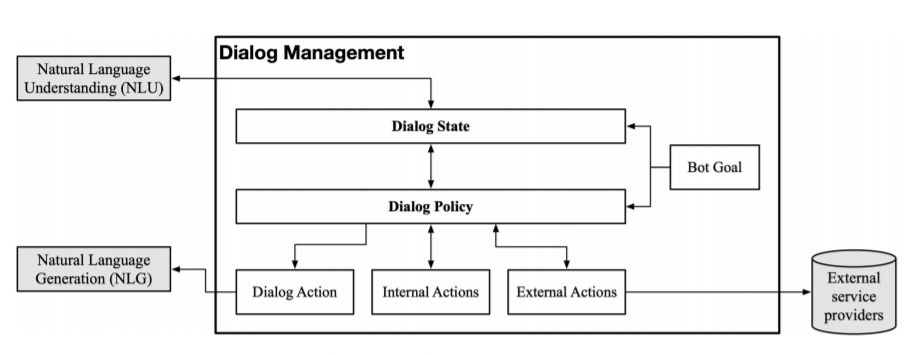
\includegraphics[width=0.9\textwidth]{img/Dialogue_Man_Sys.PNG}
    \caption{Dialogue management Architecture and information flow \cite{apprforDMS}.}
    \label{fig:dms}
\end{figure}

\subsubsection*{Communication Strategies}
Communication strategies firstly include the dialogue initiative plan. It is the basic elements that should be taken care of while designing the dialogue manager. The main goal for this interaction plan is to grant the leading role to the actors involved in a dialogue and that could be the system, user, or both. McTear et al. (2016) classified it into the following categories \cite{archDesDev}:
\begin{itemize}
    \item User-directed initiative; It happens when the user leads the communication by posting any sort of query and the system has to respond. Pros: User is not restricted and more humanly conversation. Cons: The system might not be able to respond effectively to the user's query that is not relevant to the system. It means the system can be misguided easily.
    \item System-directed initiative; The system is provided with the leading role to direct the conversation while the user is responsible for replying. Pros: Fewer chances that the system could receive deluded inputs. Cons: Limit the users and less humanly.
    \item Mixed initiative; In this approach, both are provided with the dialogue initiating rights. Pros: More real and humanly. Cons: Possibility of diverged dialogue. 
\end{itemize}
% Additionally, the dialogue manager is also responsible for error handling strategy selection for dialogue recovery.
Furthermore, another important strategy that it should adopt is the confirmation approach to make sure that the parties involved in a conversation are on the same page. McTear et al. (2016) discussed two confirmation strategies:
\begin{itemize}
    \item Explicit confirmation; System confirms again by restating the user's query as a response. Pros: Guaranteed appropriate response. Cons: Greater time complexity.
    \item Implicit confirmation; System confirms by adding the user's query in a response along with the next query. Pros: No time wastage. Cons: Chances of irrelevant response. 
\end{itemize}
McTear et al. (2016) also pitched the following examples for better understanding of confirmation strategies:
% \begin{lstlisting}[language=json,numbers=none]
\begin{itemize}
    \item Explicit Confirmation - User: "I want to go to New York." System: "You want directions to New York?" \cite{archDesDev}.
    \item Implicit Confirmation - User: "I want to go to New York." System: "What type of transportation do you want to use to get to New York?" \cite{archDesDev}.
\end{itemize}

% \end{lstlisting}
\subsubsection*{Domain}
A specific dialogue field refers to a domain. It is composed of particular actions, states, and intents required in a particular dialogue domain \cite{apprforDMS}.
% Ordered structures or sub-domains collections containing separate policy for each can be used to represent a domain 

\subsubsection*{Response Manipulation}
All responses generated using techniques mentioned before containing confidence values assigned to them. Higher the confidence, the higher the receptiveness of the response. In case of responses with lower relevancy and confidence values system should be able to respond effectively. There are the following techniques highlighted by Yu et al. (2016) used to serve this purpose \cite{stratandPolLearn}:
\begin{itemize}
    \item Topic Shifting; Instead of replying with the answer having a lower confidence index, an agent tries to divert the user by switching the context to some common interesting topic like sports, weather, or any other engaging topic. It could cause irrelevancy but users find it more logical as compared to the inappropriate response with lower confidence.
    \item Throwing Open Queries; Replacing simple fallback messages such as "I didn't understand you" etc. with some meaningful content like "Sorry, I can't say anything about it. Could you tell me something more interesting?". As both of the statements are serving the same purpose but the second statement is more helpful for dialogue continuation.
    \item Cracking a Joke; Instead of replying with an irrelevant response, a chatbot could crack a joke. It will not let the conversation stop.
    \item Additional Information Inquiry; In this technique chatbot responds with a message and asks the user to elaborate or devise his\_her query again.
\end{itemize}

\subsubsection*{Dialogue Recovery Principles}
Dialogue manager has to implement the following dialogue recovery principles stated by \cite{devPrincip}:
% are mentioned below:
% several dialogue design principles should be considered while designing a dialogue manager.  
\begin{enumerate}
    \item Disambiguation; It refers to the ability of the dialogue system to clarify the ambiguous user utterances. For example, input: “Was Amadeus nominated for an academy award?” and response: “Is Amadeus the movie's title?” \cite{archDesDev}.
    \item Relaxation; It relates to the dialogue system's capability to respond flexibly. For example, input: “Are there any flights today” and response: “No. Would
    you like me to find one tomorrow?” \cite{archDesDev}.
    \item Confirmation; Dialogue system's ability to confirm before executing critical tasks for the users. For example, response: “you want me to book you the 7 am flight from Philadelphia to San Francisco?” \cite{archDesDev}.
    \item Completion; Capability to enquire about the missing information before taking any action. For example, input: “I would like to book the 7 am flight to SF” and response: “Which airport are you flying out of?” \cite{archDesDev}.
\end{enumerate}

\subsubsection*{Dialogue Management Techniques}
Techniques used for dialogue management can be classified as (i) Handcrafted (rule-based) approaches and (ii) Probabilistic (statistical) approaches \cite{apprforDMS}.

\paragraph*{Handcrafted Approaches}
As it could be apprehended from the name of the approach that the dialogue managers implementing such a technique need the set of pre-defined rules provided by developers and domain professionals. These rules are further used to compose the system's state and policy \cite{apprforDMS}. 
\\~\\
\textit{Finite State Machines;} Dialogue managers consisted of finite-state automata, hold a single state for the conversation \cite{apprforDMS}. And with each leading transition, the state gets updated \cite{apprforDMS}. Such dialogue managers have overall control over the communication by limiting user choices.
\\~\\
\textit{Frame-based Dialogue Management;} Flexibility factor can be enhanced by adding the data model for slots tracking to the finite state machines. Such an approach is named as frame-based dialogue management \cite{apprforDMS}. Slots could get filled irrespective of any dialogue sequence empowering the user-directed initiative. 
\\~\\
\textit{Model-based Dialogue Management;} More practical approaches could be designed by appending user model, conversational model, or any related model with previously discussed data model \cite{apprforDMS}. Harms et al. (2019) provided an example of such a model and named it as an information state model. It consists of a state which is responsible to keep track of user goals and notions. It is also expected that the developer has been provided the state updating mechanism according to the possible dialogue acts \cite{apprforDMS}. 

\paragraph*{Probabilistic Approaches}
Unlike handcrafted approaches, statistical approaches are more pragmatic and possess the ability to learn the rules on their own via real conversations.
\\~\\
\textit{Example-based Method;} It was an initial statistical method that made the dialogue managers capable of getting trained using massive data collection to respond efficiently. It checks for the similarity between user utterance and the example in the data available for training purposes and selects the best response from this training corpus \cite{apprforDMS}.
\\~\\
\textit{Partially Observable Markov Decision Process(POMDP);} As explained by Harms et al. (2019), dialogue managers following such processes initially mark the dialogue state as unperceived. Secondly, there exists a state distributed over all possible states named as belief states. Whenever there comes an input it is evaluated and observed for all the possible states within a system. This observation yields the most fitting state for the user input. In the end, dialogue policy component practices reinforcement learning to take an action according to the current belief state \cite{apprforDMS}. 
\\~\\
\textit{Neural Networks;} Presently, neural networks are exercised on the dialogue managers. The main idea behind it is to omit the limitations set by handcrafted methods \cite{apprforDMS}. As such networks are composed of memory units just like humans and they are capable of reading and writing the knowledge into their memory segments. They receive the information through old and recent input provided to them.  

\paragraph*{Hybrid Approaches}
Both of the lastly mentioned dialogue management techniques have been combined and practiced to develop data-driven conversational agents \cite{apprforDMS}. Rasa Core\footnote{\url{https://legacy-docs.rasa.com/docs/core/}} is an example of such dialogue agents. And the framework developed in this master's thesis is also based upon this approach. 
\\~\\
Graphical representation of the classifications for the dialogue managers along with respective existing tools has been shown in Figure \ref{fig:dmappr}.

\begin{figure}[h]
    \centering
    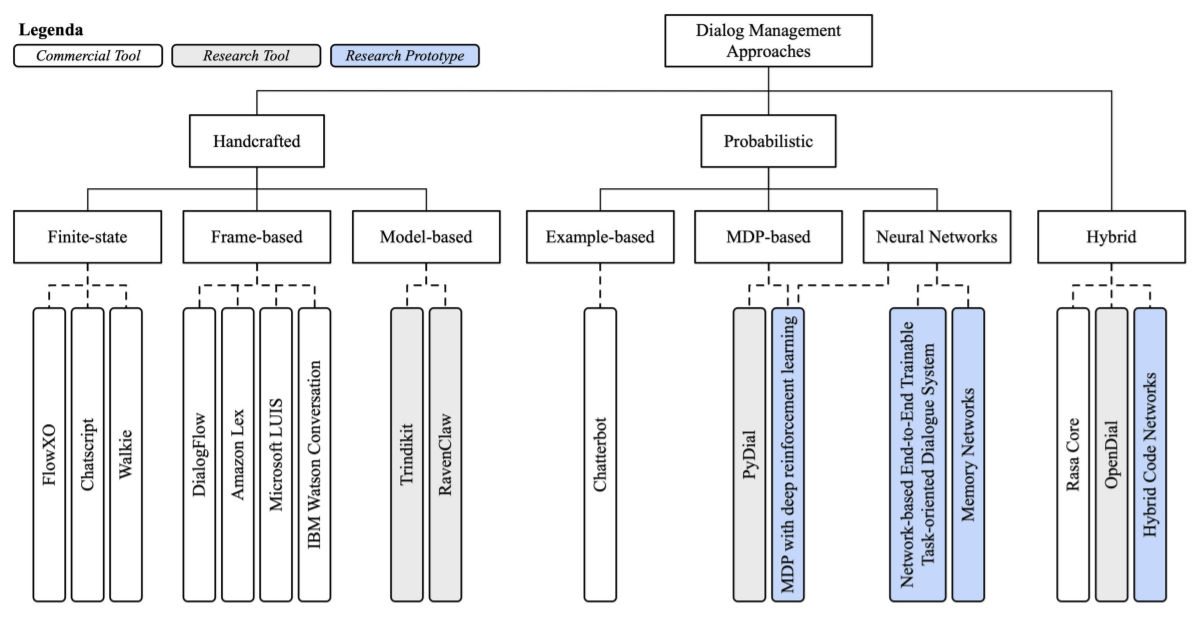
\includegraphics[width=0.9\textwidth]{img/DM_Approaches.PNG}
    \caption{Classification of Dialogue Management Approaches. Top most level shows three different approaches: handcrafted, statistical and hybrid. Next step illustrates different methods associated with each approach. Lastly, practical tools (white boxes), research tools (grey boxes), and research prototypes (blue boxes) are defined \cite{apprforDMS}.}
    \label{fig:dmappr}
\end{figure}

\subsubsection*{Challenges}
There exist few demanding factors that need to be highlighted while talking about dialogue management.
\\~\\
\textit{Coding Strategies;} Strategies used for the coding purpose are most often independent of a dialogue structure. The coding scheme and modeling strategy are responsible for the amount of information that can be delivered using a  dialogue.
\\~\\
\textit{Dialogue Structure;} Logical dialogue designing supporting state structure and transformations. Data structures like trees and graphs can be used for this purpose. While graphs can push the structure more towards complications.
\\~\\
\textit{Error Recovery;} There is a high risk of task failure but it should be made sure that dialogue must go on. It should be highly prioritized that the dialogue manager must be able to catch the errors and handle them properly. This means it should be able to recover from faulty situations using different techniques as mentioned previously under the heading "Dialogue Recovery Principles".

\section{Applications}
Cahn (2017) categorized the applications of the chatbots into the following two domains:

\subsection{Virtual Personal Assistants(VPAs)}
Virtual conversational agents are getting used extensively to assist the users at a personal level. Agents like Google Assistant, Apple's Siri, Microsoft's Cortana, and Amazon's Alexa are playing an important role in this domain \cite{archDesDev}. Such conversational agents seek command from the user and take steps accordingly to fulfill the desired task.

\subsection{User Domain-Specialist Bots}
Such bots are specialized in some user-specific domain for what they have been trained and provide instructions on user request. Some domains illustrated in \cite{archDesDev} are: (i) Transportation, (ii) Dating, (iii) Meditation, (iv) Fitness, (v) Weather and (vi) Medical.





% The task for computers, handling the knowledge progressed significantly in the 1980s under the field of "Knowledge Engineering" \cite{designandimplementation}.  
% Methods used for this purpose in the past consisted of inference tools to shape the facts and evolve new knowledge using first and second-order logic. Such techniques were used for responding efficiently to ambiguous queries. 
% \\~\\
% Knowledge engineering made the functioning easy for conversational bots. As it assists a chatbot to answer a question containing general facts \cite{designandimplementation}. Apple's Siri and Amazon's Alexa use internal knowledge inference methods to fetch the facts from the web and other users' resources \cite{designandimplementation}. 
 

% For this sub-challenge, there comes dialogue systems to rescue.





% \section{Chatbot Comparison Framework}
% based on currently introduced chatbots like Hubot, J.A.R.V.I.S., Pandorabots, Wit.ai, etc. the fundamental features vary and can be compared for virtual agents. The key elements are discussed below.

% \subsection{Types}
% According to \cite{frameworkforunderstandingchatbots} chatting assistants can differ based on the tasks that they are performing. Alertbot is a chatbot that is being used for auto-generating notification for some event that occurred. Whereas J.A.R.V.I.S. is a well-known framework for developing artificially intelligent virtual assistants that are capable of rapid self-learning and can execute engineering tasks without any human help. Referring to \cite{softwarebots} chatbot types can be classified as follows: 

% \subsubsection*{Informative}
% Such type of conversational agents are designed to help creators by grabbing the required information for some specific task. For example, to produce an alert message for any bug in a program written by some developer. 
% % \cite{frameworkforunderstandingchatbots}

% \subsubsection*{Collaborative}
% These kinds of chatbots assist the developers to collaborate and communicate efficiently to be more productive. As an example, the collaborative chatbot will alert a developer working on some project, of a chat that is started by some other developers if it involves the one who is working on it and is important for him to be notified. 
% % \cite{frameworkforunderstandingchatbots}

% \subsubsection*{Automated}
% Such chatbots work alongside the developers to provide aid in task accomplishment, having dependencies in one or more projects by detecting the problem caused due to some alteration in a feature. E.g. Auto-generated documentation.
% \cite{frameworkforunderstandingchatbots}

% \subsection{Direction}
% As mentioned earlier, chatbots differ in the objectives of the task they are performing. On the other hand, they function uni-directionally rather than taking the whole conversation into account. \cite{frameworkforunderstandingchatbots}

% \subsubsection*{Input}
% Such conversational bots search for some specific keywords or tags pushed by the creator in conversation and fire specific responses based on that keywords or phrases. They are also known as silent bots as they perform their tasks quietly. \cite{frameworkforunderstandingchatbots}

% \subsubsection*{Output}
% Output chatbots are opposite to input ones. They just need general content or an action to make them operational, unlike input bots which require some special keywords to make them trigger any output. Such kind of assistants mostly get activated from some external source and notify about events to a different place. \cite{frameworkforunderstandingchatbots}

% \subsubsection*{Bidirectional}
% Bidirectional conversational agents work in both directions. They are capable of taking an input and generating an appropriate response accordingly. It can vary from activating just a simple response for some action to real communication. \cite{frameworkforunderstandingchatbots}

% \subsection{Guidance}
% When it comes to complex chatbots, it is really important to make them function autonomously for their sustainability and practicability.

% \subsubsection*{Human Mediated}
% These kinds of chatbots require human mediation to function properly. They can't complete any task on their own. They seek the relevant information or operational directions from the developer due to which they can not cause much destruction. But if they start to do that then it is very easy for a developer to stop them from further functioning. \cite{frameworkforunderstandingchatbots}

% \subsubsection*{Autonomous}
% Chatbots which can perform their tasks on their own and contain all the viable knowledge or having the capability of self-learning lie under autonomous agents group. The only problem with such bots is that they can be invasive. \cite{frameworkforunderstandingchatbots}

% \subsection{Predictability}
% Usually, there is a group of developers responsible for designing any virtual assistant for chatting. With the diverse mindsets of developers there comes uniqueness in specifications and functionalities of a bot. So they can be distinguished based on the genre of tasks they are designed to accomplish. As stated in \cite{frameworkforunderstandingchatbots}, underneath are the following genres:

% \subsubsection*{Deterministic}
% Chatbots with the deterministic approach perform particularly the same action whenever they observe a similar event or scenario. Such communicating agents involve decision trees to make decisions based on the input provided to them. So it is easier to predict the behavior of such virtual assistants. 
% % \cite{frameworkforunderstandingchatbots}

% \subsubsection*{Evolving}
% As it is clear from the heading's name that these bots can evolve themselves. Which means they contain learning elements and can gather knowledge from past experiences and results. According to which they can regulate their actions. Which results to enhance their performance by making them capable of performing such tasks that were not instructed to them by the developer. But the drawbacks of such agents can't be ignored as they can do self-learning and can get out of control while conversation. For example, there was a chatbot for natural language multi-issue bargaining developed by Facebook. Eventually, they had to stop it because it started evolving a language that humans were unable to understand \cite{fbshutdownbot}. 
% % \cite{frameworkforunderstandingchatbots}

% \subsection{Interactivity}
% As no one can deny the fact that it is still a long time to make chatbots act like humans. But the necessity of developing human-like chatbots is rising day by day and a lot of research is happening to make chatbots interact as humans do. Although advanced chatbots can have the ability to contain more vocabulary and communicate in a much better way. It helps in enhancing the user experience and promoting chatbot's effectiveness. \cite{frameworkforunderstandingchatbots}
% \\~\\
% As claimed by \cite{frameworkforunderstandingchatbots}, there exist several styles in which chatbots interact with users as mentioned below:

% \subsubsection*{Dull}
% Chatbots with dull interaction style make conversation using common and repetitive vocabulary and chunks of words. They always use the same welcome message to greet the user without any sense to develop the new meaningful phrase with the same semantics. 

% \subsubsection*{Alternate Vocabulary}
% Such virtual agents consist of a container with multiple equivalent phrases for the same user utterance. They randomly choose the response out of a container for the utterance with the same semantics. Which makes these bots superior to dull ones. 
% % \cite{frameworkforunderstandingchatbots}

% \subsubsection*{Relationship Builder}
% Such conversational assistants try to build a good relationship with the developer or end-user. Terms used by these chatbots differ from formal to casual and vice versa. They are capable of doing continuous communication. While communicating, they can reach a point to crack a joke for humorous purposes to improve the bond and fun experience with the user. 
% % \cite{frameworkforunderstandingchatbots}

% \subsubsection*{Human-like}
% These are the most learning chatbots which use the past chat history for its training to become intelligent enough for producing appropriate response for the user query.  
% % \cite{frameworkforunderstandingchatbots}

% \begin{figure}[h]
%     \centering
%     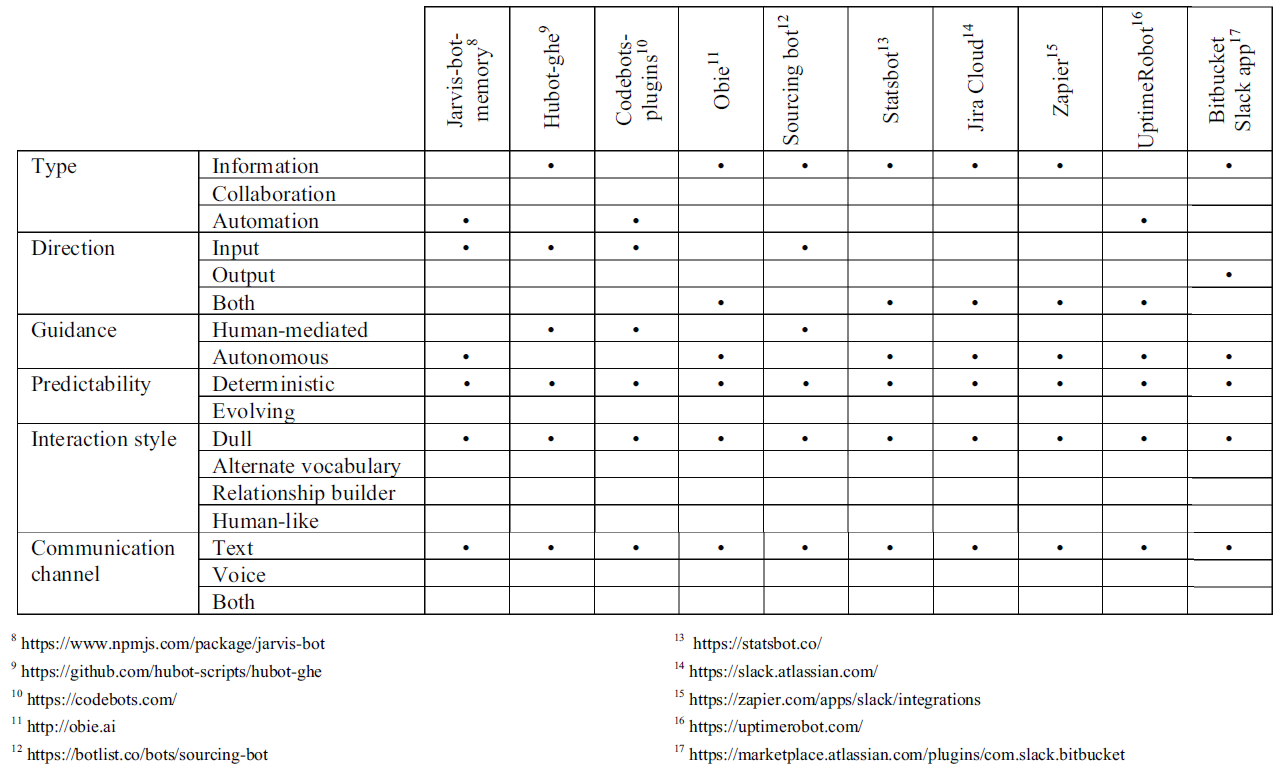
\includegraphics[width=0.9\textwidth]{img/Chatbots_Comparison_Framework.PNG}
%     \caption{Comparison framework practiced for software development on selected chatbots. \cite{frameworkforunderstandingchatbots}}
%     \label{fig:chatcompfram}
% \end{figure}



% \section{Dialogue Management Systems}
% This section covers the role, methods, and problems that occur while managing dialogue systems. They have been introduced a long time ago under the shadow of systems supporting database queries. Dialogue management systems are required for complex utterances from the user to deliver decent responses.

% \subsection{Role}
% Systems designed for dialogue management are meant to imitate conversation processing. Shaping a dialog from any source such as speech, text or any other approach is an essential step for making a dialogue manageable. If there occurs a system failure then communication must not have a full stop. The dialogue manager should be capable of catching a reason of failure and endorsing a dialogue recovery. \cite{dialoguemanagementsystems}

% \subsection{Discourse Characteristics}
% Conversation or debate between humans is not something that can be easily understandable by computers. It comprises of many complexities. But while having a dialogue between machines and humans, one can make communication using simpler language but still, a person expects that system should hold various features as claimed by \cite{dialoguemanagementsystems} are stated below: 
% \begin{itemize}
% \item \textbf{General Structure:} Dialogue consists of opening, body, and closing. Users can handle the dialogue at its opening and closing point. Whereas, the management system controls the body part of a dialogue.
% \item \textbf{Combined Initiative:} Usually user holds most of the control over a dialogue. Then there comes a system to take over the control for diminishing the misconception if there occurs any. And this task of the management system is mostly gets accomplished by verification of information provided, eliminating the confusion, or by restraining the user's reply. 
% \item \textbf{Over Gossipy:} It is in a humans nature to provide the extra useful information to others which is not even asked explicitly at that moment. The same goes with dialog management systems that they should be able to do it.
% \item \textbf{Contextual Sensation:} The system must be capable of sensing and understanding the semantics and context of the dialogue.
% \item \textbf{Error Restoration:} If there happens any error or misconception leading to dialog failure then the system should be able to restore it and not letting the conversation stop. 
% \end{itemize}

% \subsection{Modelling Dialogue Challenges}
% Following are some facts and realities of a dialogue stated in \cite{dialoguemanagementsystems}, which can not be ignored and must be taken into account while modeling a dialogue: 
% \begin{itemize}
% \item \textbf{Turn Switching:} Handling the switching of turns between user and agent or between two agents. 
% % \cite{dialoguemanagementsystems}
% \item \textbf{Conversational Fillers:} While communicating humans usually use interjections like aah! Nah!, yep! and oops!. Such words are known as fillers as they don't contain any meaning but are useful to increase the cohesiveness and convey the intentions of the user.  
% % \cite{dialoguemanagementsystems} 
% \item \textbf{Ellipsis:} Ellipsis are words omitted by humans during a conversation but can be understood using the context of previous discourse. So it is another factor that should be taken under consideration while modeling a dialogue. Otherwise, the system will not be able to deliver smartly as humans do. 
% % \cite{dialoguemanagementsystems}
% \item \textbf{Indirectness:} It involves the communication in which the literal meaning of an utterance conveys the wrong meaning. But by using intellectual capabilities, participants can interpret the correct semantics.
% % \cite{dialoguemanagementsystems}
% \item \textbf{Adjacent Dependency:} It occurs when two participants are communicating and one asks a question but the second participant instead of replying to it, posts another related question. Now it is the first one turns to respond to the question raised by the second participant to get an answer to his firstly asked question. 
% % \cite{dialoguemanagementsystems}
% \item \textbf{Anaphoric and Cataphoric Reference:} Anaphoric reference is used to get the meaning of the recent word by referring to a term used previously in the text. On the contrary, cataphoric refers to a word used afterward in the text to understand the meaning of a recently mentioned word. For example, last/next, now/then, I/you, etc.
% % \cite{dialoguemanagementsystems}
% \end{itemize}

% \subsection{Dialogue Classification}
% Classify the dialogues is not an easy task to perform. Especially when it comes to taxonomize them based on their features. The classification proposed by Dahlbäck in 1995 is based upon the tasks executed by Rubin in 1980 and Clark in 1985. According to them, dialogues can be classified under four dimensions as mentioned in \cite{dialoguemanagementsystems} are:  
% \begin{itemize}
% \item \textbf{Agent type:} It includes humans and computers with a great impact on the language used to communicate. It has been noticed that while having a conversation with virtual agents, humans use utterances more concisely, simpler, and shorter linguistics.
% \item \textbf{Communication Channel:} It underlines many distinguishing features but the most important one out of them is the method used for communication i.e. spoken or written. Other factors involve transmission styles. 
% \item \textbf{Type of Task:} It is another factor having a huge impact on the structure of the dialogue. Additionally, the task context also has a great effect. Another important aspect of having a strong impression on dialogue's structure is the number of tasks performed by a single dialogue.      
% \item \textbf{Mutual Knowledge:} Knowledge shared among the dialogue contestants also has an influence on language which can not be ignored. There exist three ways to deliver information between dialogue participants.
% \begin{enumerate}
%     \item Perception between speaker and listener.
%     \item Lingual between both.
%     \item Cultural knowledge.
% \end{enumerate} 
% \end{itemize}

% \section{Dialogue Management Techniques}
% A good dialogue management tool must include two necessary elements concerning the interaction between a user and a bot. The first one is referred to as conversation background or history for correctly determining the context of a dialogue. Whereas, the second important element is an interaction model designed to govern the system's approach for handling schema of conversation. \cite{dialoguemanagementsystems}
% \\~\\
% There exist numerous methods for artifact systems for dialogue management. But each system should include some basic components as shown in Figure \ref{fig:gsls}. Input is provided to the system as a text or interpretative speech which is further processed by natural language understanding component to infer the context and semantics. Dialogue manager is mutually connected with all components to deduce all related and meaningful related information, remove confusion and conflicts. Dialog manager's output is being used by the response generation unit to produce a response in the form of natural language or any other suitable representation may be outlined as a text to sense visually. If it is generated as a natural language then there comes a speech synthesizer to performs its task by reading it out loud for the user. \cite{dialoguemanagementsystems} 
% \begin{figure}[h]
%     \centering
%     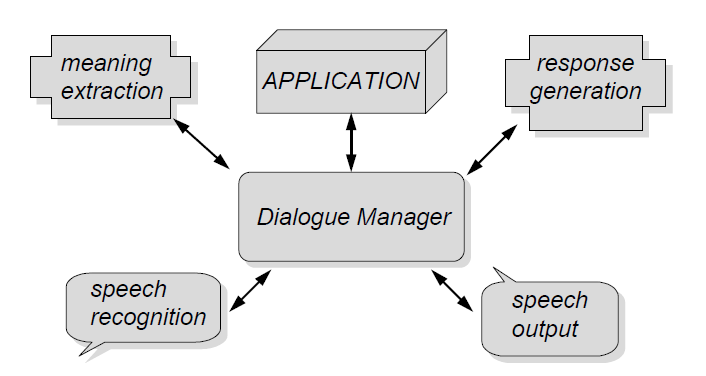
\includegraphics[width=0.9\textwidth]{img/Generic_Spoken_Language_System.PNG}
%     \caption{Generic Spoken Language Systems \cite{dialoguemanagementsystems}}
%     \label{fig:gsls}
% \end{figure}
% \\~\\
% As Figure \ref{fig:gsls} depicts just an overview of spoken dialogue systems. For more illustrative and detailed demonstration of different units along with the tasks that they are responsible for, just have a look at Figure \ref{fig:dsdm} below.
% \begin{figure}[h]
%     \centering
%     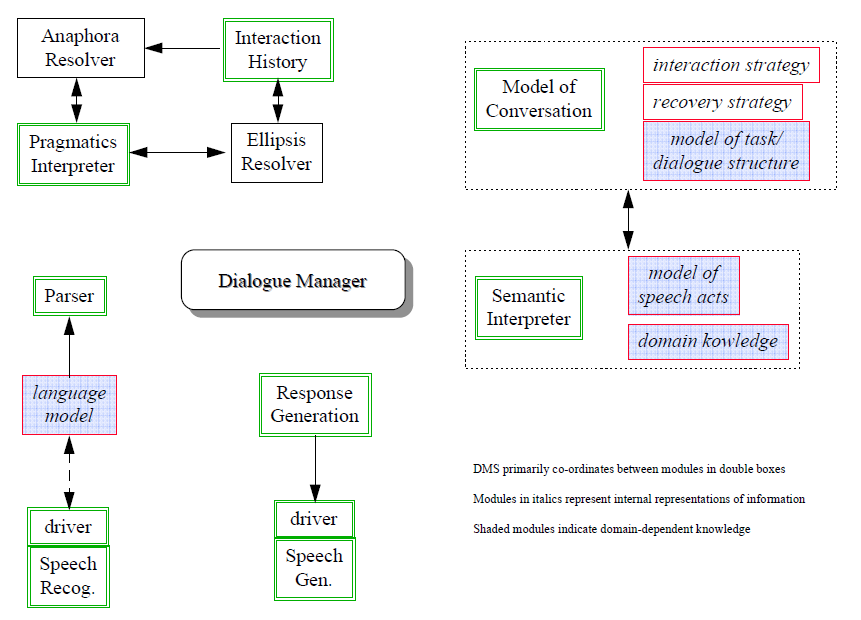
\includegraphics[width=0.9\textwidth]{img/Detailed_Spoken_Dialogue_Manager.PNG}
%     \caption{Detailed Spoken Dialogue Manager along with Key Components \cite{dialoguemanagementsystems}}
%     \label{fig:dsdm}
% \end{figure}

% \subsection{Grammars for Dialogue} 
% It is the most common initial method out of all the firstly introduced methods. It uses directed grammar from sequential sentences for dialogue description. Usually, the grammar describes the architecture of whole communication. According to \cite{dialoguemanagementsystems}, the following is the most commonly used approach for this purpose. 
% % \cite{dialoguemanagementsystems}

% \subsubsection*{Finite State Machines and Graphs}
% Finite-state models and graphical representations are the simplest methods used for managing a dialogue. The best scenario to get the full benefit out of these is when the structure of the dialogue resembles the structure of the task. Interlinked nodes join to build a graph that minimizes the user choice for selections at that very moment. And with each leading response, the state changes to another node. Like other techniques, it also has advantages along with some disadvantages. As a positive stance, the system has overall control over the communication by limiting the user choices. On the other hand, they also lack the flexibility to be adapted by some different tasks and domains. \cite{dialoguemanagementsystems} 
% \\~\\
% To overcome the flexibility issue, there come plan-based approaches to rescue.

% \subsection{Plan-based Methods}
% When it comes to complexity, these methods are considered to be more complex for dialogue designing as compared to dialogue grammars approaches. These methods are goal-specific like humans as they communicate to achieve different objectives. These methods are used to architect these goals and sub-goals for a task or dialogue. \cite{dialoguemanagementsystems}
% \\~\\
% Stated below is an application of a plan-based method taken from \cite{dialoguemanagementsystems}.

% \subsubsection*{Conversational Games Theory}
% It is a well-known pattern to develop a dialogue architecture at the mass level. In addition to that, it can also be beneficial to design a task-oriented dialogue among humans and a computer.  Both grammars from the dialogue and pattern-based approaches are involved in its development. There exists a set of rules or we can call them turns for each game. Which includes the response to some questions. So hypothetically, there exist dialogues and each dialogue is responsible to complete some small task. Which collectively results in the accomplishment of the main task. And each dialogue is responsible for performing some transactions which represent a sub-task. Whereas, every transaction represents a game associated with some conversation. 
% % \cite{dialoguemanagementsystems}

% \subsection{Collaborative Methods}
% Humans collaborate to develop some understanding among them. The main idea behind these methods is to involve both of the participants for dialogue to get a sense of mutual understanding. Collaborative techniques have the main focus on the incentive of the dialogue unlike, pattern-based approaches with having task structure as the main target. Additionally, these methods also try to grasp the dialogue structure. This means these approaches have the ability for catching general dialogue properties. \cite{dialoguemanagementsystems}

% \section{Dialogue Management Systems: Challenges}
% There exist two major concerns for a dialogue management system. The first one includes the coding strategy for the design and structure of a system. Secondly, the recovery technique to overcome a particular error is also a challenging task.

% \subsection{Coding Strategies}
% Strategies used for the coding purpose are most often independent of a dialogue structure. They are usually used to design conversation using a deterministic approach i.e. finite state machine, or non-deterministic approach i.e. statistical model. The coding scheme and modeling strategy are responsible for the amount of information that can be delivered using a dialogue. There are different types of techniques that can be useful under different circumstances. But the basic need is to understand the user's point of view from the utterance which is a challenging task. And for a better understanding of a user's intention, support can be taken from the context. So for this purpose, a linguistic philosopher Austin in 1962 initiated the research which was later named Speech Acts Theory after the contributions by Searle in 1969. \cite{dialoguemanagementsystems}  

% \subsubsection*{Speech Acts}
% Austin initiated it after noticing that some user utterances are not only the statements but can be an order to perform some action. He demonstrated the following two sentences to make it more understandable:
% \begin{enumerate}
%     \item “I bet you sixpence it will rain tomorrow”
%     \item “I name this ship Queen Elizabeth”
% \end{enumerate} 
% These statements can not only be judged as true or false. So he classified such statements as Performative Statements. Whereas, those statements that can be examined using true/false flags were named as Constative Statements.
% \\~\\
% Later, the classification proposed by Austin was proven wrong. As both types mentioned before can be put under the shadow of illocutionary acts. Illocutionary reflects the true purpose of the statement that can be an offering, promise, or a warning. This illocutionary act was named as "Speech Act". Which demonstrates the true view of the user utterance. 
% \\~\\
% With its applications, a problem was raised when the identified act doesn't match the intended user act. To overcome the problem, the identification of a perlocutionary act is important. For example, "It is cold in here" seems not to be a statement but a request to turn on the heat or any other related appeal. So, Searle in 1975 declared it as another type of speech act Indirect Speech Act(ISA). But it made the automatic labeling a real problematic task due to the uncertainty of the utterance that if it should be considered literal or interpreted. 
% \\~\\
% Furthermore, Brown and Yule in 1983, proposed another problem with speech acts while applying them to user utterances. Speech acts need a one-to-one mapping between user utterance and an act. But there can be a scenario where multiple user utterances are responsible to complete a speech act or multiple speech acts can be performed with the help of a single utterance.
% \\~\\
% Considering above mentioned problems with speech acts, Bunt in 1989 came up with another approach to succeed speech acts and that was Dialogue Interpretation Theory(DIT). According to this theory, the dialogues can be classified under two categories: a task-oriented for controlling a dialogue and proposed content integration. \cite{dialoguemanagementsystems}

% \subsubsection*{Dialogue Structure}
% A dialogue having an independent domain can add some structure to a dialogue while getting converted to dependent morphology. But the structure added is limited to the general acts. As mentioned above, conversational game theory adds a dialogue structure on top of the speech act.
% \\~\\
% Another methodology of adding a structure to dialogue was introduced by Alexandersson in 1996. It takes a collection of dialogues followed by dialogue acts to produce an intentional structure for itself. This means dialogue is divided into goals and sub-goals to gain a structure with some hierarchy. This process can be completed using the following three steps as stated by \cite{dialoguemanagementsystems}\cite{automaticacquisition}: 
% \begin{enumerate}
%     \item Acts in a collection are traversed to convert them to domain-independent from dependent hierarchy.
%     \item Encapsulate dialogue sequences in different classes. Which are responsible for some functionality or representing a dialogue phase.
%     \item Auto-production of context-free-grammar using the Bayesian Model.
% \end{enumerate} 

% \subsection{Error Recovery}
% There is a high risk of task failure but it should be made sure that dialogue must go on. It should be highly prioritized that the dialogue manager must be able to catch the error and handle it properly. Which means it should be able to recover from such faulty situations. The bugs can vary from speech recognition to inaccurate semantic analysis of the user's utterance. For this purpose, a manager must encounter it correctly and undergo some appropriate strategy. So, the taken action may differ depending upon the scenario. It must follow the recursive pattern to detect errors that occurred while solving the old one. \cite{dialoguemanagementsystems}
% \\~\\
% While handling speech recognition, mainly following three types of errors are generated as referred by \cite{communicationaldeviation}\cite{pragmaticinterpretation}: 
% \begin{itemize}
% \item \textbf{Uncertainty:} It occurs when there is low confidence for speech input.
% \item \textbf{Inconsistency:} It refers to misconception or misunderstanding. This means the input speech holds high confidence value but opposes the former conversation.       
% \item \textbf{Ambiguity:} It occurs when the system gets confused between more than one high confidence values for speech input.
% \end{itemize} 
% \\~\\
% Luperfoy proposed the following four steps recovery method in 1996 as stated by \cite{tutoringversustraining}\cite{dialoguemanagementsystems}: 
% \begin{itemize}
% \item \textbf{Detection:} Error detection is a challenging task and can also be user dependent to inform the system about it.
% \item \textbf{Diagnosis:} It includes error classification.       
% \item \textbf{Selecting Repair Plan:} It depends upon the diagnosed error class.
% \item \textbf{Executing Interactive Plan:} Selected recovery plan should be executed in an interactive manner to fairly deal with the errors produced by the plan executed.
% \end{itemize}

\section{Evaluation Methods}
Once the dialogue system is developed and ready to be launched, it must be undergone through some evaluation techniques. It never has been an easy task to evaluate dialogue systems. Usually, its complexity depends upon the criteria of what to evaluate and how to evaluate it. In addition to that, assessment is also dependent on different features. The ability of a system to auto-recover itself in case of any error is known as robustness. It should be assessed beforehand during the implementation of a system. The other essential thing to evaluate is the effectiveness of a system that is, how effective, acceptable, and friendly a system is for managing a dialogue. According to \cite{dialoguemanagementsystems}, there are two of the following methods already being introduced i.e. Quantitative and Qualitative Approaches.

\subsection{Qualitative Methods}
It can be inferred from the name that such methods are used to evaluate the quality of the conversational assistant. These methods involve users to get the mission accomplished. So users' opinions play a major role to make assessment decisions for a system. 
\\~\\
For carrying it out, once the users have adopted and utilized a system, they are provided with a questionnaire to fill or an interview can be conducted for them with different questions regarding the performance of a system. Which also includes the questions about performance, natural behavior, user-friendliness of the system, and how well it performed under certain circumstances. It also varies from person to person that some persons respond positively whilst others can provide negative impressions. Even though the system is the same based on different user preferences. So, it is better to make a user well familiar with a system first and then ask him/her to give an opinion.
\\~\\
Some interviews had been conducted by Dybkjaer in 1995 after making the users familiar with a system that can be found in \cite{qualitativeevaluation}.

\subsection{Quantitative Methods}
To assess a dialogue system quantitatively, already two techniques have been introduced so far i.e. black box and glass box. 

\subsubsection*{Black Box Testing}
It is based upon the input and the respective output without caring about the design and other internal structure of a system. It is just an outer level or top-level evaluation and can be performed by the end-user.

\subsubsection*{Glass Box Testing}
In this type of assessment, the system's internal individual components can be evaluated. And for this purpose, a developer must have the data from the past so that the current output of a component can be compared with the previous one. Such a comparison can provide one with information about the accuracy of a virtual dialogue agent. Such testing can't be performed using a black box technique as there is no trustful data available for comparing a dialogue. \cite{dialoguemanagementsystems}

\subsection{Cross-systems Comparison}
In addition to the above-mentioned evaluation techniques, there also exist some other methodologies to evaluate the dialogue management systems such as objective performance evaluation. It is recommended to perform an objective evaluation for the dialogue to make its performance compared with other management systems. Also in the present era, there are several states of the art chatbots available like IBM Watson, etc. One can also easily evaluate self-created chatbots by doing comparison after designing the same dialogue on any other state of the art virtual assistants.

\subsection{Evaluation Metrics}
Also, there are following evaluation metrics used to quantify the performance of a chatbot according to \cite{differentMeasurementsMetrics}:
\begin{itemize}
\item Dialogue efficiency metrics in terms of matching type.
\item Dialogue quality metrics based on the response type.
\item Users' satisfaction assessment metrics.
\end{itemize}

\subsection{Standard AttrakDiff Tool}
AttrakDiff is a standardized tool designed to measure the attractiveness(usability and design) of an interactive product \cite{attrakdiff}. It provides the results gathered about the hedonic and pragmatic quality of the system. Both hedonic, as well as pragmatic qualities, have a great influence on the attractiveness of the system \cite{inflOfHedandPrag}.
\\~\\
As shown in Figure \ref{fig:attrakMod} that attractiveness is based upon pragmatic and hedonic qualities of the system. Furthermore, hedonic quality is divided into two categories in the current version of the AttrakDiff: (i) Identification (HQ-I) and (ii) Stimulation (HQ-S). Pragmatic quality(PQ) includes the usability of the system i.e. the system delivered for what it has been designed. And as a consequence of PQ, user satisfaction gets collected \cite{PqHq}. Whereas, HQ-I is associated with the way products communicate important personal values as compared to other relevant products. Moreover, HQ-S is an extent to which a product is perceived as challenging or novel. 

\begin{figure}[H]
    \centering
    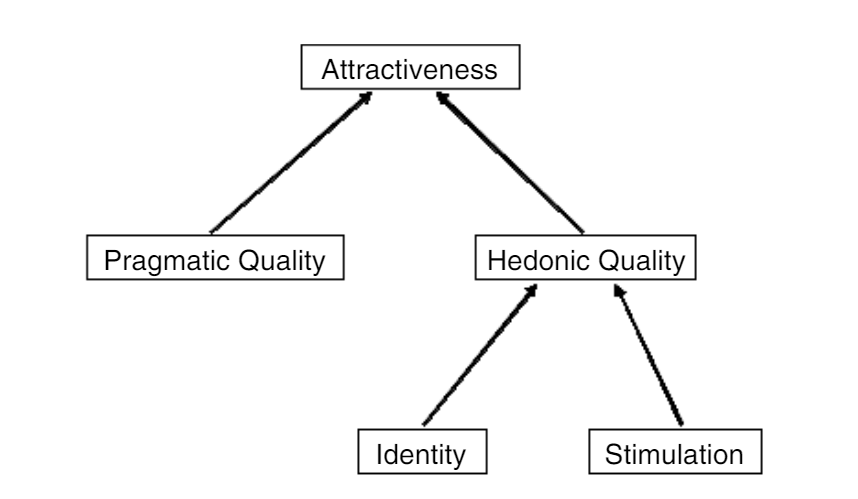
\includegraphics[width=0.7\textwidth]{img/AttrakDiff_Model.PNG}
    \caption{Main Concept of the AttrakDiff's Model \cite{inflOfHedandPrag}.}
    \label{fig:attrakMod}
\end{figure}
\\~\\
The next chapter illustrates the system architecture and overview of the chatbot named as "Frankenbot" along with its capabilities.

